% =====================================================================
% NOTE DE RECHERCHE — Calibrage et simulation du GSE IRCANTEC
% Représentation autorégressive agrégée à régime latent commun :
% estimation par maximum de vraisemblance jointe et simulation cohérente.
% Cadre GENERAL : aucune corrélation fixée a priori ; toute la dépendance
% est estimée librement, par régime, sur les résidus standardisés.
% Charte Nexialog v2 (mai 2026). Polices Montserrat + Source Sans Pro
% avec repli automatique (Times + Helvetica) si non installées.
% Compilation : pdflatex (x2). Document autonome (logo en repli texte).
% =====================================================================
\documentclass[11pt,a4paper]{article}

% --------- PACKAGES ---------------------------------------------------
\usepackage[utf8]{inputenc}
\usepackage[T1]{fontenc}
\IfFileExists{sourcesanspro.sty}{\usepackage[default]{sourcesanspro}}{\usepackage{mathptmx}}
\IfFileExists{montserrat.sty}{\usepackage{montserrat}}{\usepackage[scaled=0.92]{helvet}}
\usepackage{microtype}
\usepackage{cmap}
\usepackage{geometry}
\usepackage{graphicx}
\usepackage{xcolor}
\usepackage{amsmath,amssymb,amsthm,mathtools,bm}
\usepackage{textcomp}
\usepackage{fancyhdr}
\usepackage{titlesec}
\usepackage[hyperref]{etoc}
\usepackage{enumitem}
\usepackage{tcolorbox}
\usepackage{xurl}
\usepackage{hyperref}
\usepackage{booktabs}
\usepackage{colortbl}
\usepackage{array}
\usepackage{longtable}
\usepackage{float}
\usepackage{caption}
\usepackage{tabularx}
\usepackage{tikz}
\usetikzlibrary{arrows.meta,positioning,calc,fit,backgrounds}
\usepackage{needspace}
\usepackage{etoolbox}

% --------- CHARTE NEXIALOG (officielle v2) ----------------------------
\definecolor{nxnavy}{HTML}{002060}
\definecolor{nxred}{HTML}{B10031}
\definecolor{nxteal}{HTML}{409ABB}
\definecolor{nxslate}{HTML}{223E55}
\definecolor{nxgray}{HTML}{9A999E}
\definecolor{nxlightgray}{HTML}{D0D1D4}
\definecolor{nxoffwhite}{HTML}{F2F2F2}
\definecolor{nxgreen}{HTML}{2E7D32}
\definecolor{nxorange}{HTML}{F57C00}
\definecolor{nxlightblue}{HTML}{E6ECF7}

% --------- LOGO (repli texte si le PDF est absent) -------------------
\newcommand{\nxlogo}[1][0.50\textwidth]{%
  \IfFileExists{logo_nexialog.pdf}%
    {\includegraphics[width=#1]{logo_nexialog.pdf}}%
    {\parbox{#1}{\centering\sffamily\bfseries\color{nxnavy}\fontsize{30}{34}\selectfont NEXIALOG\\[1mm]{\normalsize\color{nxred}\,CONSULTING}}}}
\newcommand{\nxlogosmall}{%
  \IfFileExists{logo_nexialog.pdf}%
    {\includegraphics[height=13mm]{logo_nexialog.pdf}}%
    {\sffamily\bfseries\color{nxnavy}\large NEXIALOG\,{\color{nxred}\small C.}}}

% --------- PAGE SETUP -------------------------------------------------
\geometry{a4paper, top=32mm, bottom=22mm, left=25mm, right=25mm,
          headheight=19mm, headsep=6mm}

% --------- HEADER / FOOTER --------------------------------------------
\pagestyle{fancy}
\fancyhf{}
\fancyhead[L]{\parbox[c][14mm][c]{52mm}{\nxlogosmall}}
\fancyhead[R]{\parbox[c][14mm][c]{110mm}{\raggedleft\small GSE IRCANTEC~~\textbar~~\textit{Note de recherche --- Calibrage \& simulation}}}
\fancyfoot[L]{\small Note de recherche --- Juin 2026}
\fancyfoot[R]{\small Page \thepage}
\renewcommand{\headrulewidth}{0pt}
\renewcommand{\footrulewidth}{0.3pt}
\renewcommand{\footrule}{\hbox to\headwidth{\color{nxlightgray}\leaders\hrule height \footrulewidth\hfill}}

% --------- STYLES DE SECTION (Montserrat) -----------------------------
\titleformat{\section}{\sffamily\Large\bfseries\color{nxnavy}}{\thesection.}{0.5em}{}
\titleformat{\subsection}{\sffamily\large\bfseries\color{nxnavy}}{}{0em}{\thesubsection.~}
\titleformat{\subsubsection}{\sffamily\normalsize\bfseries\color{nxnavy}}{}{0em}{\thesubsubsection.~}

% --------- TABLE DES MATIÈRES (etoc) ----------------------------------
\etocsetstyle{section}{}{}
  {\par\noindent\sffamily\large\bfseries\textcolor{nxred}{\etocname}\hfill\textcolor{nxred}{\etocpage}\par\medskip}{}
\etocsetstyle{subsection}{}{}
  {\par\noindent\hspace*{5mm}\sffamily\normalsize\mdseries\textcolor{nxnavy}{\etocname}\hfill\textcolor{nxnavy}{\etocpage}\par\vspace{6pt}}{}
\etocsetstyle{subsubsection}{}{}
  {\par\noindent\hspace*{10mm}\sffamily\small\mdseries\textcolor{nxnavy}{\etocname}\hfill\textcolor{nxnavy}{\etocpage}\par\vspace{5pt}}{}
\etocsettocstyle{}{}

% --------- ENVIRONNEMENTS PERSONNALISÉS -------------------------------
\tcbuselibrary{skins,breakable}
\newtcolorbox{definitionbox}[1][]{enhanced, breakable,
  colback=nxlightblue, frame hidden, boxrule=0pt, arc=3pt,
  before skip=4mm, after skip=3mm, left=4mm, right=4mm, top=3mm, bottom=3mm}

\newtcolorbox{insightbox}[1][Point clé]{enhanced, breakable,
  colback=nxoffwhite, frame hidden, boxrule=0pt, arc=3pt,
  fonttitle=\sffamily\bfseries\color{nxred}, title={#1},
  detach title, before upper={\tcbtitle\par\nobreak\medskip\nobreak},
  before skip=4mm, after skip=3mm, left=4mm, right=4mm, top=3mm, bottom=3mm}

\newtcolorbox{mabox}[1][]{enhanced, breakable,
  colback=nxlightblue, frame hidden, boxrule=0pt, arc=3pt,
  fonttitle=\sffamily\bfseries\color{nxnavy}, title={#1},
  detach title, before upper={\tcbtitle\par\nobreak\medskip\nobreak},
  before skip=4mm, after skip=3mm, left=4mm, right=4mm, top=3mm, bottom=3mm}

\newtcolorbox{algobox}[1][Algorithme]{enhanced, breakable,
  colback=white, colframe=nxnavy, boxrule=0.8pt, arc=3pt,
  fonttitle=\sffamily\bfseries\color{white}, coltitle=white,
  colbacktitle=nxnavy, title={#1},
  before skip=4mm, after skip=3mm, left=4mm, right=4mm, top=3mm, bottom=3mm}

\theoremstyle{definition}
\newtheorem{proposition}{Proposition}
\newtheorem{remarque}{Remarque}

% --------- CAPTIONS / FLOATS ------------------------------------------
\captionsetup{font=small,labelfont={bf,color=nxnavy},labelsep=period}
\setlength{\abovecaptionskip}{4pt}\setlength{\belowcaptionskip}{4pt}
\setlength{\textfloatsep}{10pt plus 2pt minus 2pt}
\setlength{\floatsep}{8pt plus 2pt minus 2pt}
\setlength{\intextsep}{10pt plus 2pt minus 2pt}
\renewcommand{\topfraction}{0.92}\renewcommand{\bottomfraction}{0.92}
\renewcommand{\textfraction}{0.05}\renewcommand{\floatpagefraction}{0.85}
\widowpenalty=10000\clubpenalty=10000

% --------- LISTES & ANTI-ORPHELINS ------------------------------------
\setlist{leftmargin=*, labelindent=0pt, itemsep=2pt, topsep=4pt}
\pretocmd{\section}{\needspace{6\baselineskip}}{}{}
\pretocmd{\subsection}{\needspace{5\baselineskip}}{}{}
\pretocmd{\subsubsection}{\needspace{4\baselineskip}}{}{}
\BeforeBeginEnvironment{definitionbox}{\needspace{5\baselineskip}}
\BeforeBeginEnvironment{insightbox}{\needspace{5\baselineskip}}
\BeforeBeginEnvironment{mabox}{\needspace{4\baselineskip}}
\BeforeBeginEnvironment{algobox}{\needspace{6\baselineskip}}

% --------- HYPERREF ---------------------------------------------------
\hypersetup{colorlinks=true, linkcolor=nxred, citecolor=nxred, urlcolor=nxred,
  linktoc=all, pdftitle={Note de recherche -- Calibrage et simulation du GSE IRCANTEC},
  pdfauthor={Nexialog Consulting}}

% --------- OPÉRATEURS / RACCOURCIS MATH -------------------------------
\DeclareMathOperator{\Corr}{Corr}
\DeclareMathOperator{\Var}{Var}
\DeclareMathOperator{\Cov}{Cov}
\DeclareMathOperator{\diag}{diag}
\DeclareMathOperator{\tr}{tr}
\DeclareMathOperator{\chol}{chol}
\DeclareMathOperator{\vecop}{vec}
\DeclareMathOperator*{\argmin}{arg\,min}
\DeclareMathOperator*{\argmax}{arg\,max}
\newcommand{\R}{\mathbb{R}}
\newcommand{\E}{\mathbb{E}}
\newcommand{\Prob}{\mathbb{P}}
\newcommand{\Ecal}{\mathcal{E}}
\newcommand{\Ncal}{\mathcal{N}}
\newcommand{\Xcal}{\mathcal{X}}
\newcommand{\eps}{\varepsilon}
\newcommand{\transp}{^{\!\top}}
\newcommand{\dd}{\mathrm{d}}
\newcommand{\Dt}{\Delta}

\setlength{\emergencystretch}{2.5em}
\tolerance=1200

% =====================================================================
\begin{document}
% =====================================================================

% --------- PAGE DE GARDE ----------------------------------------------
\begin{titlepage}
\thispagestyle{empty}
\vspace*{-5mm}
\begin{center}\nxlogo[0.55\textwidth]\end{center}
\vspace{1.4cm}
\begin{center}
  {\color{nxred}\rule{0.6\textwidth}{1.5pt}}\\[10mm]
  {\sffamily\bfseries\color{nxnavy}\fontsize{24pt}{30pt}\selectfont
   \MakeUppercase{Calibrage et simulation du GSE}\\[4mm]
   \MakeUppercase{Représentation autorégressive}\\[2mm]
   \MakeUppercase{à régime latent commun}}\\[10mm]
  {\color{nxred}\rule{0.6\textwidth}{1.5pt}}\\[10mm]
  {\sffamily\large\color{nxnavy}Note de recherche méthodologique}\\[3mm]
  {\sffamily\normalsize\color{nxnavy}Juin 2026}
\end{center}
\vspace{10mm}
\noindent\begin{minipage}{\textwidth}\small
Cette note de recherche est un document \textbf{autonome} consacré à l'\emph{estimation} et à la \emph{simulation} du générateur de scénarios économiques (GSE) monde réel du régime IRCANTEC. Elle ne reprend ni le diagnostic critique, ni les volets \emph{courbe des taux}, \emph{pricing} zéro-coupon, prime de liquidité ou \emph{smoothing} : on s'y limite, pour chaque facteur de risque, au \emph{modèle de diffusion} et à sa \emph{discrétisation} (exacte ou approchée, au pas $\Dt$), puis on construit un \textbf{unique modèle autorégressif agrégé} à régime latent commun regroupant tous les facteurs.

\vspace{2mm}
Le cadre est \textbf{général} : aucune corrélation n'est fixée \emph{a priori} (ni à zéro, ni à dire d'expert). Toute la dépendance --- entre facteurs, à l'intérieur d'un facteur vectoriel, et selon le régime --- est \emph{estimée librement} sur les résidus standardisés. L'objet central est la \textbf{méthodologie de calibrage par maximum de vraisemblance jointe} (et non par appariement de moments ni régression \emph{ad hoc}), déclinée en une procédure séquentielle en trois étapes --- marges, régime commun, corrélations par régime --- avec \emph{formes fermées explicites} partout où elles existent, puis la \textbf{technique de simulation} cohérente associée. Le dernier chapitre applique le cadre à un AR regroupant l'intégralité des facteurs et en donne toutes les \emph{expressions littérales finales}, directement implémentables. Document confidentiel, à usage méthodologique exclusif de l'IRCANTEC et de la Caisse des Dépôts.
\end{minipage}
\vfill
\begin{center}{\sffamily\bfseries\large\color{nxnavy}THINK SMART~~\textcolor{nxred}{$\bullet$}~~ACT DIFFERENT}\end{center}
\end{titlepage}

% --------- TABLE DES MATIÈRES -----------------------------------------
\begingroup
\hypersetup{hidelinks}
\vspace*{\stretch{0.5}}
{\noindent\sffamily\Huge\bfseries\color{nxnavy}Table des matières\par}
\vspace{16mm}
\tableofcontents
\vspace*{\stretch{2}}
\endgroup
\newpage

% =====================================================================
\section{Objet et périmètre}

Le générateur de scénarios économiques (GSE) du régime simule par Monte-Carlo, sur un horizon ALM d'une trentaine d'années, l'ensemble des facteurs de risque qui alimentent l'allocation stratégique. Chaque facteur obéit à une équation différentielle stochastique (EDS) propre, que l'on discrétise au pas mensuel avant de la simuler. Cette note traite deux maillons de cette chaîne~: d'une part, nous montrons que tous les facteurs se mettent sous une \emph{forme autorégressive unique}~; d'autre part, nous proposons une méthodologie de \emph{calibrage} et une \emph{simulation cohérente} de cette représentation.

\begin{insightbox}[Fil directeur]
Une fois discrétisée, toute EDS du GSE devient une récurrence autorégressive vectorielle dont les coefficients peuvent dépendre du pas $\Dt$ et d'un \emph{régime de marché commun} $\Ecal_t$. Nous agrégeons les facteurs en un \emph{unique} modèle vectoriel à changement de régime (MS-VAR), nous le calibrons facteur par facteur puis pour la dépendance (procédure séquentielle de type IFM), et nous le simulons directement à partir de cette même représentation. L'estimation et la simulation reposent ainsi sur une seule loi, et aucune corrélation n'est imposée~: toute la dépendance est estimée.
\end{insightbox}

\noindent Pour chaque facteur, nous ne rappelons que son modèle de diffusion et sa discrétisation. Les traitements amont --- valorisation de la courbe nominale, corrections de covariance zéro-coupon, prime de liquidité, déslissage (\emph{unsmoothing}) --- ne sont pas abordés~: nous travaillons sur les séries de facteurs qui en résultent. Nous nous limitons enfin à la structure de diffusion (dérive, retour à la moyenne, positivité, régime) et n'imposons aucune contrainte sur les (co)variances de bruit~: la matrice de dépendance reste libre et se trouve estimée par régime, y compris la corrélation interne d'un facteur vectoriel.

% =====================================================================
\section{Notations}
\label{sec:notations}
% =====================================================================
Le pas est mensuel, $\Dt=1/12$, et les facteurs sont observés aux dates $t_k=k\Dt$ ($k=0,\dots,n$, avec $n\approx240$), de trajectoire $Y_{0:n}=(Y_{t_0},\dots,Y_{t_n})$. Les facteurs sont indexés par $i$ et les régimes par $a,b\in\{1,\dots,K\}$. L'état global $Y_t\in\R^{d}$ ($d=\sum_i d_i=12$) empile les états $Y^{(i)}_t\in\R^{d_i}$ ($d_i=2$ pour un Vasicek bi-factoriel, $1$ sinon)~; $D=3$ actifs portent le régime.

Le régime $\Ecal_t\in\{1,\dots,K\}$ suit une chaîne de Markov de transition $p_{ab}=\Prob(\Ecal_{t+\Dt}=b\mid\Ecal_t=a)$, $P=(p_{ab})$, et de loi invariante $\pi$ solution de $\pi\transp P=\pi\transp$, $\sum_a\pi_a=1$.

Les innovations $\eps_{t+\Dt}\in\R^d$ sont standardisées ($\Ncal(0,1)$ par composante) et corrélées par $\Omega(\Ecal_t)$~: $\eps_{t+\Dt}=L(\Ecal_t)z_{t+\Dt}$ avec $z_{t+\Dt}\sim\Ncal(0,I_d)$ et $L(a)L(a)\transp=\Omega(a)$. La récurrence du facteur $i$ s'écrit $Y^{(i)}_{t+\Dt}=\Phi_i\,Y^{(i)}_t+c_i+D_i\,\eps^{(i)}_{t+\Dt}$, de matrice autorégressive $\Phi_i$, constante $c_i$ et échelle $D_i$ (\S\ref{sec:ar}).

On note $\Phi$ et $\varphi$ la f.d.r.\ et la densité de $\Ncal(0,1)$, $\varphi_p(\cdot;m,V)$ la densité $\Ncal(m,V)$ en dimension $p$, $F_{\chi'^2}(\cdot;\nu,\lambda)$ la f.d.r.\ du $\chi^2$ décentré, et $f_i(\cdot\mid Y^{(i)}_t,\Ecal_t;\theta)$ (resp.\ $F_i$) la densité (resp.\ f.d.r.) de transition exacte du facteur $i$, c.-à-d.\ $F_i(y\mid Y^{(i)}_t,\Ecal_t)=\Prob\big(Y^{(i)}_{t+\Dt}\le y\mid Y^{(i)}_t,\Ecal_t\big)$~; $\hat\theta$ désigne les paramètres estimés et $\ell$ la log-vraisemblance. Les paramètres et quantités propres à chaque facteur sont définis avec son modèle (\S\ref{sec:facteurs}) et sa procédure d'estimation (\S\ref{sec:calib}).

% =====================================================================
\section{Modèles de diffusion et discrétisation}
\label{sec:facteurs}
% =====================================================================
Nous rappelons, pour chaque famille de facteurs, l'EDS de diffusion et sa discrétisation au pas $\Dt$, qui est exacte sauf mention contraire et n'impose aucune restriction sur les corrélations.

\subsection{Taux nominaux et réels : Vasicek à deux facteurs (V2F)}
\label{sec:v2f}
Un facteur court $q^s_t$ revient vers un facteur long stochastique $q^l_t$, qui lui-même retourne vers une cible de long terme $\mu$, selon
\[
\dd q^s_t=\kappa_1(q^l_t-q^s_t)\dd t+\sigma_1\dd W^1_t,\qquad
\dd q^l_t=\kappa_2(\mu-q^l_t)\dd t+\sigma_2\dd W^2_t,\quad \dd\langle W^1,W^2\rangle=\rho\,\dd t .
\]
En posant $X_t=(q^s_t,q^l_t)\transp$, $A=\bigl(\begin{smallmatrix}\kappa_1&-\kappa_1\\0&\kappa_2\end{smallmatrix}\bigr)$ et $\Sigma_w=\bigl(\begin{smallmatrix}\sigma_1^2&\rho\sigma_1\sigma_2\\\rho\sigma_1\sigma_2&\sigma_2^2\end{smallmatrix}\bigr)$, le système s'écrit $\dd X_t=A(\mu_\infty-X_t)\dd t+\Sigma_w^{1/2}\dd W_t$ avec $\mu_\infty=(\mu,\mu)\transp$. Sa loi de transition conditionnelle est gaussienne exacte, $X_{t+\Dt}\mid X_t\sim\Ncal\big(\Phi X_t+(I-\Phi)\mu_\infty,\ \Sigma_{\mathrm{cond}}\big)$, soit~:
\begin{definitionbox}
\[
X_{t+\Dt}=\Phi X_t+(I-\Phi)\mu_\infty+\eta_{t+\Dt},\qquad \eta_{t+\Dt}\sim\Ncal(0,\Sigma_{\mathrm{cond}}),
\]
où $\Phi=e^{-A\Dt}=\bigl(\begin{smallmatrix}e^{-\kappa_1\Dt}&\phi_{12}\\0&e^{-\kappa_2\Dt}\end{smallmatrix}\bigr)$, $\phi_{12}=\tfrac{\kappa_1}{\kappa_1-\kappa_2}(e^{-\kappa_2\Dt}-e^{-\kappa_1\Dt})$, et $\Sigma_{\mathrm{cond}}=\Sigma_\infty-\Phi\Sigma_\infty\Phi\transp=\bigl(\begin{smallmatrix}V_r&C_{mr}\\C_{mr}&V_m\end{smallmatrix}\bigr)$ avec $\Sigma_\infty$ solution de l'équation de Lyapunov $A\Sigma_\infty+\Sigma_\infty A\transp=\Sigma_w$.
\end{definitionbox}
\noindent La corrélation conditionnelle $\rho_c=C_{mr}/\sqrt{V_r V_m}$ demeure libre, car elle est portée par $\Omega$ et non fixée. Les taux réels suivent la même structure, en remplaçant $(q^s,q^l)$ par $(r,l)$.

\subsection{Crédit \emph{investment grade} : spread CIR}
Le spread $s_t$ suit une diffusion à racine carrée, $\dd s_t=\kappa(\theta-s_t)\dd t+\sigma\sqrt{s_t}\,\dd W_t$, qui garantit la positivité. Sa loi de transition est exacte mais non gaussienne~: en posant $c_\chi=\tfrac{2\kappa}{\sigma^2(1-e^{-\kappa\Dt})}$, la variable $2c_\chi s_{t+\Dt}\mid s_t$ suit un $\chi^2$ décentré de paramètres $\nu=\tfrac{4\kappa\theta}{\sigma^2}$ et $\lambda=2c_\chi s_te^{-\kappa\Dt}$. Lorsqu'on préfère un schéma explicite et positif, on retient le schéma d'Alfonsi $E(0)$, valable sous $\sigma^2\le4\kappa\theta$~:
\[
\bar s_{t+\Dt}=\Big((1-\tfrac{\kappa}{2}\Dt)\sqrt{\bar s_t}+\tfrac{\sigma\,\Dt W_t}{2(1-\frac{\kappa}{2}\Dt)}\Big)^2+(\kappa\theta-\tfrac{\sigma^2}{4})\Dt .
\]

\subsection{Dette privée : log-Vasicek (Black--Karasinski)}
Le logarithme du spread suit un Ornstein--Uhlenbeck, $\dd\ln s_t=k(\theta-\ln s_t)\dd t+\sigma\dd W_t$, ce qui maintient le spread strictement positif. La loi de transition conditionnelle est gaussienne exacte, $y_{t+\Dt}\mid y_t\sim\Ncal\big(e^{-k\Dt}y_t+\theta(1-e^{-k\Dt}),\ \tfrac{\sigma^2}{2k}(1-e^{-2k\Dt})\big)$, soit~:
\[
y_{t+\Dt}=e^{-k\Dt}y_t+\theta(1-e^{-k\Dt})+\sigma\sqrt{\tfrac{1-e^{-2k\Dt}}{2k}}\,\eps_{t+\Dt},\qquad y=\ln s,\ \eps\sim\Ncal(0,1),
\]
de loi stationnaire $\ln s_\infty\sim\Ncal(\theta,\sigma^2/2k)$.

\subsection{Actions cotées : changement de régime de Hardy (RSLN-2)}
Conditionnellement au régime $\Ecal_t$, les rendements suivent un Black--Scholes, $\dd S_t/S_t=\mu_{\Ecal_t}\dd t+\sigma_{\Ecal_t}\dd W_t$. Le log-rendement se discrétise alors exactement, de loi conditionnelle au régime $x_{t+\Dt}\mid\{\Ecal_t=a\}\sim\Ncal(m_a,v_a)$, soit $x_{t+\Dt}=m_{\Ecal_t}+\sqrt{v_{\Ecal_t}}\,\eps_{t+\Dt}$ avec $m_a=(\mu_a-\tfrac{\sigma_a^2}{2})\Dt$ et $v_a=\sigma_a^2\Dt$. C'est le seul facteur dont les coefficients de marge dépendent du régime.

\subsection{Actifs à valorisation espacée (PE, immobilier, infrastructure) : Black--Scholes}
Après déslissage, les rendements suivent un Black--Scholes à coefficients constants, dont le log-rendement se discrétise exactement par $x_{t+\Dt}=m+\sqrt{v}\,\eps_{t+\Dt}$, avec $m=\mu\Dt$ et $v=\sigma^2\Dt$, où $\mu$ est la dérive en log annualisée (monde réel, sans correction de convexité). Les log-rendements sont alors indépendants et gaussiens. Ces facteurs peuvent être promus au Groupe~B (régime propre) si les données le justifient (\S\ref{sec:msvar}).

\begin{table}[H]
\centering\small\renewcommand{\arraystretch}{1.25}\setlength{\tabcolsep}{6pt}
\begin{tabularx}{\textwidth}{@{}l l c c@{}}
\toprule
\textbf{Facteur} & \textbf{Diffusion} & \textbf{Discrétisation} & \textbf{Exacte ?}\\
\midrule
\rowcolor{nxlightblue} Inflation, taux réels & Vasicek 2 facteurs & gaussienne bivariée & Oui\\
Crédit IG & CIR & $\chi^2$ décentré / Alfonsi & Loi exacte~; schéma Alfonsi approché\\
\rowcolor{nxlightblue} Dette privée & Black--Karasinski & gaussienne (log-spread) & Oui\\
Actions (Euro/Monde/Émerg.) & Hardy RSLN-2 & BS par régime & Oui (cond.\ régime)\\
\rowcolor{nxlightblue} PE / Immo / Infra & Black--Scholes & log-rendement gaussien & Oui\\
\bottomrule
\end{tabularx}
\caption{Modèle et discrétisation de chaque facteur. Cinq familles sur six admettent une discrétisation exacte~; seul le CIR demande un schéma positif approché (Alfonsi), alors que sa loi exacte reste simulable.}
\label{tab:disc}
\end{table}

% =====================================================================
\section{Représentation autorégressive commune}
\label{sec:ar}
% =====================================================================
Toutes les discrétisations du Tableau~\ref{tab:disc} partagent une même structure, que nous écrivons pour chaque facteur $i$ sous la forme
\begin{definitionbox}
\[
\boxed{\;Y^{(i)}_{t+\Dt}=\Phi_i(\Ecal_t)\,Y^{(i)}_t+c_i(\Ecal_t)+D_i(\Ecal_t)\,\eps^{(i)}_{t+\Dt}\;}
\]
où $\eps^{(i)}$ est l'innovation standardisée, $\Phi_i$ la matrice autorégressive, $c_i$ le terme déterministe et $D_i$ l'échelle conditionnelle. Toute corrélation est reportée dans la matrice $\Omega(\Ecal_t)$.
\end{definitionbox}
\noindent Cette écriture partitionne les facteurs selon la dépendance de leurs \emph{marges} au régime~: le Groupe~A rassemble les facteurs dont les coefficients $\{\Phi_i,c_i,D_i\}$ ne dépendent pas de $\Ecal$, le Groupe~B ceux dont ils en dépendent. La partition est configurable, puisqu'un facteur Black--Scholes peut être promu au Groupe~B. Elle ne concerne toutefois que les marges~: la dépendance $\Omega(\Ecal_t)$ reste libre et propre au régime pour tous les facteurs.

\begin{table}[H]
\centering\small\renewcommand{\arraystretch}{1.4}
\begin{tabularx}{\textwidth}{@{}l l X c@{}}
\toprule
\textbf{Facteur} & \textbf{Forme AR} & \textbf{Coefficients (marge)} & \textbf{Gr.}\\
\midrule
V2F & VAR(1) gaussien $2{\times}2$ & $\Phi=e^{-A\Dt}$, $D=\diag(\sqrt{V_r},\sqrt{V_m})$ & A\\
Black--Karasinski & AR(1) sur $y=\ln s$ & $\Phi=e^{-k\Dt}$, $c=\theta(1-e^{-k\Dt})$, $D=\sigma\sqrt{\tfrac{1-e^{-2k\Dt}}{2k}}$ & A\\
CIR & AR « racine carrée » non linéaire & $\sqrt{\bar s_{t+\Dt}}\approx|a\sqrt{\bar s_t}+b\,\Dt W|$, bruit gaussien & A\\
Hardy RSLN-2 & AR(0) par régime & $\Phi=0$, $c(\Ecal)=m_\Ecal$, $D(\Ecal)=\sqrt{v_\Ecal}$ & B\\
BS déslissé & AR(0) gaussien & $\Phi=0$, $c=\mu\Dt$, $D=\sigma\sqrt{\Dt}$ & A$^{(\dagger)}$\\
\bottomrule
\end{tabularx}
\caption{Mise sous forme AR de chaque facteur, où $(V_r,V_m)=\diag(\Sigma_{\mathrm{cond}})$ pour le V2F. Le symbole $^{(\dagger)}$ rappelle qu'un BS est promouvable au Groupe~B. Le CIR n'étant pas affine en $s$, sa récurrence est non linéaire mais son bruit reste gaussien~; $\rho_c$ et toutes les corrélations croisées résident dans $\Omega(\Ecal_t)$.}
\label{tab:formes}
\end{table}

% =====================================================================
\section{Résidus standardisés et copule}
\label{sec:pit}
% =====================================================================
Pour traiter de façon homogène les facteurs gaussiens et non gaussiens et pour isoler proprement la dépendance, nous standardisons chaque innovation par transformée intégrale de probabilité (PIT). Concrètement, nous transformons chaque composante en un score gaussien~:
\begin{definitionbox}
\[
\widehat\eps^{(j)}_{t+\Dt}=\Phi^{-1}\big(F_j(Y^{(j)}_{t+\Dt}\mid Y_t,\Ecal_t;\hat\theta)\big),
\]
où $F_j(y\mid Y_t,\Ecal_t)=\Prob\big(Y^{(j)}_{t+\Dt}\le y\mid Y_t,\Ecal_t\big)$ est la f.d.r.\ conditionnelle marginale de la composante $j$. Sous bonne spécification, $\widehat\eps^{(j)}$ est i.i.d.\ $\Ncal(0,1)$.
\end{definitionbox}
\noindent Pour une composante gaussienne (V2F, BK, BS, ou Hardy conditionnellement au régime), cette transformation se réduit à une division par l'écart-type conditionnel~; nous ne blanchissons pas le bloc, de sorte que les corrélations conditionnelles, dont $\rho_c$ du V2F, restent portées par $\Omega$. Pour le CIR, $F_j$ est la f.d.r.\ du $\chi^2$ décentré.

La dépendance prend alors la forme d'une copule sur ces scores~: $\widehat\eps_{t+\Dt}\sim\Ncal(0,\Omega(\Ecal_t))$, où $\Omega$ est pleine, libre et propre au régime, et s'estime sur les résidus plutôt que sur les niveaux. Nous contrôlons l'adéquation a posteriori (uniformité des PIT, normalité, queues)~; lorsque les queues l'exigent, une copule de Student, de matrice d'échelle $\Omega(\Ecal_t)$ et de marges restituées $\Ncal(0,1)$, est disponible en option.

% =====================================================================
\section{Modèle agrégé à régime commun (MS-VAR)}
\label{sec:msvar}
% =====================================================================
Nous empilons enfin tous les facteurs en un unique modèle vectoriel à changement de régime~:
\begin{definitionbox}
\[
\boxed{\;Y_{t+\Dt}=c(\Ecal_t)+\Phi(\Ecal_t)Y_t+D(\Ecal_t)\eps_{t+\Dt},\quad \eps_{t+\Dt}\sim\Ncal(0,\Omega(\Ecal_t)),\quad \Ecal_t\sim\text{Markov}(P)\;}
\]
où $\Phi(a)$, $c(a)$ et $D(a)$ sont bloc-diagonaux par facteur --- constants en $a$ pour le Groupe~A, fonction de $a$ pour le Groupe~B --- et $\Omega(a)$ est la corrélation pleine et propre au régime.
\end{definitionbox}
\noindent La dépendance repose ainsi sur deux mécanismes non imposés~: la chaîne $\Ecal_t$ porte le co-mouvement systémique (entrée conjointe en stress) et la matrice $\Omega(\Ecal_t)$ la dépendance intra-régime. Le rattachement d'un facteur au Groupe~B relève d'un choix de configuration.

% =====================================================================
\section{Méthodologie de calibrage}
\label{sec:calib}
% =====================================================================

\subsection{Un cadre de calibrage des marges méthode-agnostique}
Chaque facteur possédant une densité de transition exacte (Tableau~\ref{tab:disc}), nous pouvons en principe calibrer chaque marge par maximum de vraisemblance conditionnelle,
\[
\hat\theta_i=\argmax_{\theta\in\Theta_i}\ \sum_t\log f_i\big(Y^{(i)}_{t+\Dt}\mid Y^{(i)}_t,\Ecal_t;\theta\big),
\]
où $\Theta_i$ est le domaine admissible des paramètres ($\kappa>0$, $\sigma>0$, stationnarité). Cet estimateur, efficient et atteignant la borne de Cramér--Rao, constitue notre choix par défaut. Le cadre reste néanmoins général~: selon le facteur, plusieurs méthodes coexistent et sont sélectionnables --- l'EMV, les moindres carrés (MCO), l'appariement de moments, ou les cibles distributionnelles.

\noindent L'estimation conjointe directe de toutes les marges, de la chaîne et de toutes les corrélations serait numériquement fragile (grande dimension, multimodalité). Nous adoptons donc la procédure séquentielle de type IFM (\emph{Inference Functions for Margins}) illustrée à la Figure~\ref{fig:cascade}, qui est consistante, modulaire et stable~: nous estimons d'abord les marges du Groupe~A, puis le régime commun et les marges du Groupe~B, et enfin la dépendance par régime.

\begin{figure}[H]
\centering
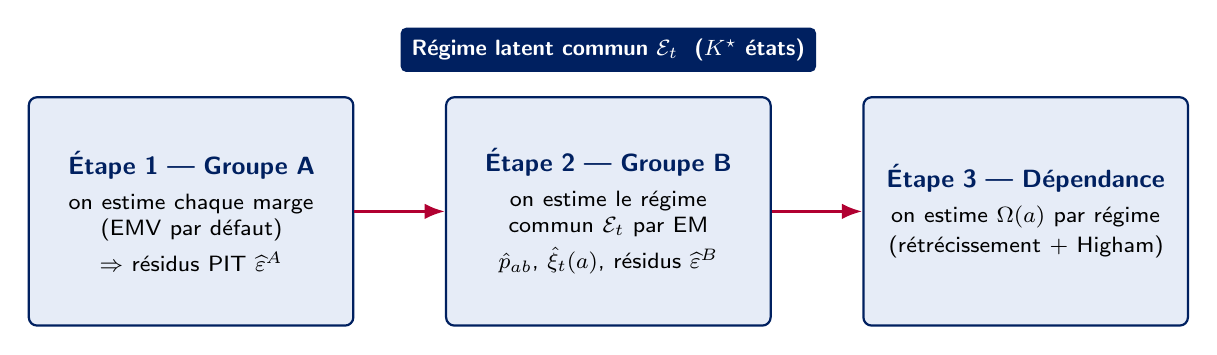
\begin{tikzpicture}[font=\sffamily\small,
  box/.style={rectangle, rounded corners=3pt, draw=nxnavy, line width=0.8pt, fill=nxlightblue, text width=3.7cm, align=center, inner sep=6pt, minimum height=2.9cm},
  lab/.style={rectangle, rounded corners=2pt, fill=nxnavy, text=white, inner sep=4pt, font=\sffamily\footnotesize\bfseries},
  arr/.style={-{Latex[length=2.6mm,width=2.0mm]}, line width=1.1pt, draw=nxred}]
\node[box] (a) {\textbf{\textcolor{nxnavy}{Étape 1 --- Groupe A}}\\[3pt]\footnotesize on estime chaque marge\\ (EMV par défaut)\\[2pt] $\Rightarrow$ résidus PIT $\widehat\eps^A$};
\node[box, right=1.15cm of a] (b) {\textbf{\textcolor{nxnavy}{Étape 2 --- Groupe B}}\\[3pt]\footnotesize on estime le régime\\ commun $\Ecal_t$ par EM\\[2pt] $\hat p_{ab}$, $\hat\xi_t(a)$, résidus $\widehat\eps^B$};
\node[box, right=1.15cm of b] (c) {\textbf{\textcolor{nxnavy}{Étape 3 --- Dépendance}}\\[3pt]\footnotesize on estime $\Omega(a)$ par régime\\ (rétrécissement $+$ Higham)};
\node[lab, above=3mm of b] (top) {Régime latent commun $\Ecal_t$ \ ($K^\star$ états)};
\draw[arr] (a) -- (b);
\draw[arr] (b) -- (c);
\end{tikzpicture}
\caption{Cascade séquentielle (IFM). L'Étape~1 estime chaque marge par la méthode choisie, l'Étape~2 itère l'EM (à ascension monotone), et l'Étape~3 estime toutes les corrélations par régime, sans contrainte.}
\label{fig:cascade}
\end{figure}

\subsection{Étape 1 --- marges du Groupe A}
Pour chaque facteur $i\in A$, nous estimons $\hat\theta_i$ par la méthode retenue (\S\ref{sec:closed}), puis nous en déduisons les résidus PIT $\widehat\eps^{(i)}$. La propriété IFM garantit la consistance de ces marges indépendamment de la dépendance croisée.

\subsection{Étape 2 --- régime commun par EM}
Les actions (Groupe~B) partagent un même régime caché $\Ecal_t\in\{1,\dots,K\}$. À chaque date $t=1,\dots,n$ nous observons leur vecteur de log-rendements $x_t\in\R^{D}$~; nous notons $x_{1:n}=(x_1,\dots,x_n)$ la séquence observée et $x_{1:t}=(x_1,\dots,x_t)$ son préfixe jusqu'à $t$. Conditionnellement au régime, l'émission est gaussienne, de densité conditionnelle
\[
f_a(x)=\varphi_D(x;m_a,V_a),\qquad f_a(x)\,\dd x=\Prob\!\big(x_t\in[x,x+\dd x]\mid\Ecal_t=a\big).
\]
Nous estimons $(m_a,V_a)_{a}$, $P$ et $\pi$ par l'algorithme EM, qui alterne un pas~E (probabilités de régime) et un pas~M (paramètres). Le pas~E met en jeu quatre probabilités conditionnelles, que nous définissons avant de les calculer~:
\[
\xi_{t\mid t-1}(a)=\Prob(\Ecal_t=a\mid x_{1:t-1}),\qquad
\xi_{t\mid t}(a)=\Prob(\Ecal_t=a\mid x_{1:t}),
\]
\[
\hat\xi_t(a)=\Prob(\Ecal_t=a\mid x_{1:n}),\qquad
\hat\xi_t(a,b)=\Prob(\Ecal_t=a,\,\Ecal_{t+1}=b\mid x_{1:n}),
\]
respectivement \emph{prédite} (au vu du passé strict), \emph{filtrée} (au vu du passé), \emph{lissée} et \emph{jointe lissée} (au vu de tout l'échantillon).

\paragraph{Pas E.} Le \emph{filtre de Hamilton}, initialisé par $\xi_{1\mid0}=\hat\pi$, calcule par récurrence avant la probabilité prédite puis la filtrée~:
\[
\xi_{t\mid t-1}(a)=\sum_b\xi_{t-1\mid t-1}(b)\,p_{ba},\qquad
\xi_{t\mid t}(a)=\frac{\xi_{t\mid t-1}(a)\,f_a(x_t)}{\sum_{a'}\xi_{t\mid t-1}(a')\,f_{a'}(x_t)},
\]
et fournit au passage la log-vraisemblance $\ell=\sum_t\log\!\big(\sum_a\xi_{t\mid t-1}(a)\,f_a(x_t)\big)$. Le \emph{lisseur de Kim}, initialisé par $\hat\xi_n=\xi_{n\mid n}$, parcourt ensuite les dates à rebours et en déduit les probabilités lissées~:
\[
\hat\xi_t(a)=\sum_b\hat\xi_{t+1}(b)\,\frac{\xi_{t\mid t}(a)\,p_{ab}}{\xi_{t+1\mid t}(b)},\qquad
\hat\xi_t(a,b)=\hat\xi_{t+1}(b)\,\frac{\xi_{t\mid t}(a)\,p_{ab}}{\xi_{t+1\mid t}(b)}.
\]

\paragraph{Pas M.} Le pas M met à jour les paramètres en forme fermée~:
\[
\hat m_a=\frac{\sum_t\hat\xi_t(a)x_t}{\sum_t\hat\xi_t(a)},\quad
\hat V_a=\frac{\sum_t\hat\xi_t(a)(x_t-\hat m_a)(x_t-\hat m_a)\transp}{\sum_t\hat\xi_t(a)},\quad
\hat p_{ab}=\frac{\sum_t\hat\xi_t(a,b)}{\sum_t\hat\xi_t(a)} .
\]
La covariance $\hat V_a$ est pleine, ce qui revient à estimer sans contrainte les corrélations intra-régime du Groupe~B. L'algorithme garantit l'ascension monotone de la vraisemblance~; nous imposons des planchers de variance pour écarter les optima dégénérés et nous ordonnons les régimes par volatilité décroissante (le régime~1 désigne ainsi le stress). La loi invariante, qui sert à l'initialisation et à la simulation, résout $\hat\pi\transp\hat P=\hat\pi\transp$ avec $\sum_a\hat\pi_a=1$.

\subsection{Étape 3 --- dépendance par régime}
\label{sec:etape3}
Une fois les marges figées, nous mesurons la corrélation des résidus séparément dans chaque régime, nous la stabilisons par rétrécissement, puis nous la rendons définie-positive afin de pouvoir simuler. En notant $\widehat\eps_t\in\R^d$ le vecteur complet des résidus standardisés, la cible est la corrélation conditionnelle au régime, $\Omega(a)=\E\big[\widehat\eps_{t+\Dt}\widehat\eps_{t+\Dt}\transp\mid\Ecal_t=a\big]$ (une matrice de corrélation, les marges étant $\Ncal(0,1)$). À marges fixées, son estimateur du maximum de vraisemblance de la copule gaussienne est la moyenne empirique pondérée par les probabilités lissées $\hat\xi_t(a)$~:
\begin{definitionbox}
\[
\widehat\Omega(a)=\frac{\sum_t\hat\xi_t(a)\,\widehat\eps_t\widehat\eps_t\transp}{\sum_t\hat\xi_t(a)},\qquad a=1,\dots,K^\star .
\]
\end{definitionbox}
\noindent Un masque de sensibilité $S\in\{0,1\}^{d\times d}$ permet de rendre certaines corrélations communes aux régimes~: on pose $\widehat\Omega(a)_{ij}=S_{ij}\,G^{\mathrm{reg}}_{ij}(a)+(1-S_{ij})\,G^{\mathrm{pool}}_{ij}$ hors diagonale, où $G^{\mathrm{reg}}(a)$ est la corrélation pondérée ci-dessus et $G^{\mathrm{pool}}=\tfrac1n\sum_t\widehat\eps_t\widehat\eps_t\transp$ la corrélation poolée. Comme un régime peu peuplé donne une corrélation quasi singulière en échantillon fini, nous rétrécissons $\widehat\Omega(a)$ vers la cible poolée,
\[
\widehat\Omega^{\mathrm{sh}}(a)=(1-\delta_a)\widehat\Omega(a)+\delta_a\,G^{\mathrm{pool}},\qquad
\delta_a=\min\!\Big(\tfrac{d}{n^{\mathrm{eff}}_a},1\Big),\qquad
n^{\mathrm{eff}}_a=\frac{(\sum_t\hat\xi_t(a))^2}{\sum_t\hat\xi_t(a)^2},
\]
où $n^{\mathrm{eff}}_a$ est la taille d'échantillon effective de Kish. Nous projetons enfin la matrice sur le cône des corrélations définies-positives par l'algorithme de Higham, $\Omega^{\mathrm{SDP}}(a)=\textsc{NearestCorr}(\widehat\Omega^{\mathrm{sh}}(a))$, ce qui rend possible la décomposition de Cholesky $L(a)L(a)\transp=\Omega^{\mathrm{SDP}}(a)$. Toutes les entrées --- intra-V2F, intra-Groupe~B et croisées --- sont ainsi estimées, jamais imposées.

\subsection{Estimateurs des marges}
\label{sec:closed}
Nous donnons à présent l'estimateur de chaque famille, avec ses variantes éventuelles.

\paragraph{Ornstein--Uhlenbeck scalaire (Black--Karasinski).}
Pour la récurrence $y_{t+\Dt}=\beta y_t+\theta(1-\beta)+\xi$ avec $\xi\sim\Ncal(0,v)$ et $\beta=e^{-k\Dt}$, l'EMV maximise la vraisemblance gaussienne sous les contraintes $\beta\in(0,1)$ et $\sigma>0$~; à l'intérieur de ce domaine, il admet la forme fermée des moindres carrés~:
\begin{definitionbox}
\[
\hat\beta=\frac{\sum_t(y_t-\bar y_-)(y_{t+\Dt}-\bar y_+)}{\sum_t(y_t-\bar y_-)^2},\quad
\hat\theta=\frac{\bar y_+-\hat\beta\bar y_-}{1-\hat\beta},\quad
\hat k=-\frac{\ln\hat\beta}{\Dt},\quad
\hat\sigma=\sqrt{\hat v\,\tfrac{-2\ln\hat\beta}{\Dt(1-\hat\beta^2)}} .
\]
\end{definitionbox}
Si $\hat\beta$ sort de $(0,1)$, cette forme fermée quitte le domaine admissible et c'est l'EMV sous contrainte qui prévaut. Lorsque la moyenne est imposée, on régresse sans constante sur $(y-\theta_0)$.

\paragraph{Vasicek à deux facteurs --- trois méthodes.}
La discrétisation est un VAR(1) gaussien $Y_{t+\Dt}=c(\theta)+\Phi(\theta)Y_t+\eta$ de bruit $\eta\sim\Ncal(0,\Sigma_{\mathrm{cond}}(\theta))$, dont les coefficients $c(\theta)=(I-\Phi)(\mu,\mu)\transp$, $\Phi(\theta)=e^{-A\Dt}$ et $\Sigma_{\mathrm{cond}}(\theta)=\Sigma_\infty-\Phi\Sigma_\infty\Phi\transp$ (avec $\vecop(\Sigma_\infty)=(I\otimes A+A\otimes I)^{-1}\vecop(\Sigma_w)$) sont des fonctions exactes de $\theta=(\kappa_1,\kappa_2,\sigma_1,\sigma_2,\rho,\mu)$. Nous proposons trois méthodes d'estimation, sélectionnables et comparées à la référence (tableau~\ref{tab:res-v2f-meth}).

\emph{(i) EMV séquentiel} (\texttt{mle}, défaut). Comme le facteur long est autonome, nous procédons en deux temps. Nous estimons d'abord le facteur \emph{long} seul, par l'EMV de l'Ornstein--Uhlenbeck scalaire, ce qui fournit $(\hat\kappa_2,\hat\sigma_2,\hat\mu)$ que nous figeons. Nous estimons ensuite le facteur \emph{court} par l'EMV du vecteur $(q^s,q^l)$, les paramètres du long restant fixés, sur les seuls $(\kappa_1,\sigma_1,\rho)$~:
\begin{definitionbox}
\[
(\hat\kappa_1,\hat\sigma_1,\hat\rho)=\argmax_{\kappa_1,\sigma_1,\rho}\ \sum_t\log\varphi_2\big(Y_{t+\Dt};c(\theta)+\Phi(\theta)Y_t,\Sigma_{\mathrm{cond}}(\theta)\big),\qquad (\kappa_2,\sigma_2,\mu)\text{ figés}.
\]
\end{definitionbox}
Nous menons les deux étapes sur le domaine admissible. La séquence estime ainsi explicitement la corrélation $\rho$ des browniens court--long, et rend $\kappa_2$ robuste puisqu'il provient de l'OU scalaire, ce qui évite la dégénérescence d'un EMV pleinement joint.

\emph{(ii) MCO en cascade} (\texttt{ols}). Nous estimons la forme réduite par moindres carrés~: le long par un OU autonome, puis $q^s$ régressé sur $(1,q^s_t,q^l_t)$. Nous en déduisons $\hat\kappa_i=-\Dt^{-1}\ln\widehat\Phi_{ii}$ et lisons $\hat\rho_c$ sur $\widehat\Sigma_{\mathrm{cond}}$~; les volatilités structurelles s'obtiennent par une inversion OU par facteur, approchée. Cette méthode est rapide mais peut sortir du domaine admissible.

\emph{(iii) Cibles distributionnelles} (\texttt{distributional}), décrites au paragraphe suivant.

\paragraph{Vasicek à deux facteurs --- cibles distributionnelles.}
Plutôt que la vraisemblance, cette méthode choisit $(\kappa_1,\kappa_2,\sigma_1,\sigma_2)$ pour que le modèle reproduise trois statistiques observées des taux ($\mu$ étant fixé ou estimé par régression, et les browniens supposés indépendants, $\Sigma_w=\diag(\sigma_1^2,\sigma_2^2)$). Sous l'hypothèse des espérances, le taux de maturité $\tau$ est affine en les facteurs, $R(t,t+\tau)=\mu+\tfrac1\tau[B_1(\tau)(q^s_t-\mu)+B_2(\tau)(q^l_t-\mu)]$, avec
\[
B_1(\tau)=\!\int_0^\tau\!e^{-\kappa_1 s}\dd s=\tfrac{1-e^{-\kappa_1\tau}}{\kappa_1},\qquad
B_2(\tau)=\!\int_0^\tau\!\phi_{12}(s)\dd s=\tfrac{\kappa_1}{\kappa_1-\kappa_2}\Big(\tfrac{1-e^{-\kappa_2\tau}}{\kappa_2}-\tfrac{1-e^{-\kappa_1\tau}}{\kappa_1}\Big),
\]
où $B_2$ est l'intégrale du coefficient de transmission $\phi_{12}$ (\S\ref{sec:v2f}), et nous notons $B_{ik}=B_k(\tau_i)/\tau_i$ la matrice de chargement. À partir de la covariance stationnaire des facteurs $\Sigma^X_\infty$ (Lyapunov), de celle de leurs incréments $\Sigma^{\Delta X}_\infty=2\Sigma^X_\infty-\Phi\Sigma^X_\infty-\Sigma^X_\infty\Phi\transp$, et de leurs images sur les taux $\Sigma^Y_\infty=B\Sigma^X_\infty B\transp$ et $\Sigma^{\Delta Y}_\infty=B\Sigma^{\Delta X}_\infty B\transp$, nous formons les trois cibles du modèle (volatilité des variations, corrélation entre maturités, dispersion des niveaux) et les ajustons à leurs analogues historiques~:
\begin{definitionbox}
\[
(\hat\kappa,\hat\sigma)=\argmin_{\kappa,\sigma>0}\
\tfrac{\lambda_v}{m}\!\sum_i\!\Big(\tfrac{\sigma^{\mathrm{mod}}_{\Delta Y}(\tau_i)}{\sigma^{\mathrm{hist}}_{\Delta Y}(\tau_i)}-1\Big)^2
+\tfrac{2\lambda_c}{m(m-1)}\!\sum_{i<j}\!\big(\rho^{\mathrm{mod}}_{\Delta Y}-\rho^{\mathrm{hist}}_{\Delta Y}\big)^2
+\tfrac{\lambda_s}{m}\!\sum_i\!\Big(\tfrac{\sigma^{\mathrm{mod}}_{Y}(\tau_i)}{\sigma^{\mathrm{hist}}_{Y}(\tau_i)}-1\Big)^2,
\]
\end{definitionbox}
où $\sigma^{\mathrm{mod}}_{\Delta Y}(\tau_i)=\sqrt{(\Sigma^{\Delta Y}_\infty)_{ii}/\Dt}$, $\rho^{\mathrm{mod}}_{\Delta Y}=(\Sigma^{\Delta Y}_\infty)_{12}/\sqrt{(\Sigma^{\Delta Y}_\infty)_{11}(\Sigma^{\Delta Y}_\infty)_{22}}$ et $\sigma^{\mathrm{mod}}_{Y}(\tau_i)=\sqrt{(\Sigma^{Y}_\infty)_{ii}}$. L'écart-type historique des niveaux se corrige du biais d'autocorrélation par $\sigma^{\mathrm{hist}}_Y=\sqrt{\widehat\Omega^2}$ avec $\widehat\Omega^2=\big(\tfrac1n\sum_k(Y_{t_k}-\bar Y)^2\big)/\big(1-\tfrac1{n^2}\sum_{l}(n-|l|)\rho^Y_\infty(l\Dt)/\rho^Y_\infty(0)\big)$, l'autocorrélation $\rho^Y_\infty$ étant celle du modèle ($\Gamma_Y(l)=B\,\Phi^{l}\Sigma^X_\infty B\transp$), donc bornée. Cet objectif est mal posé~: lorsque $\kappa_1$ croît, le chargement du facteur court $B_1(\tau)/\tau\sim1/(\kappa_1\tau)$ tend vers zéro et le facteur court se découple, ce qui crée une crête $\sigma^2/\kappa$. Nous la levons en ajoutant une régularisation ridge faible $\varrho\sum_i(\ln\kappa_i-\ln\kappa^{\mathrm{ols}}_i)^2$. Cette méthode est celle de la référence~; elle restitue des volatilités plus élevées que l'EMV. Les résidus et la simulation identifient toutefois les facteurs aux taux observés, comme pour \texttt{mle} et \texttt{ols}~: l'estimation distributionnelle ne fournit que les paramètres de marge.

\paragraph{Black--Scholes (PE, immobilier, infrastructure).}
Nous déslissons d'abord les rendements par la transformation de Lizieri, $r^\ast_t=(r_t-\hat b\,r_{t-1})/(1-\hat b)$, où $\hat b$ est le coefficient AR(1) estimé par MCO de $r_t$ sur $r_{t-1}$. Les log-rendements étant ensuite i.i.d.\ $\Ncal(m,v)$, l'estimateur est $\hat m=\tfrac1n\sum x_t$, $\hat v=\tfrac1n\sum(x_t-\hat m)^2$ et $\hat\sigma=\sqrt{\hat v/\Dt}$. En cadre monde réel, nous retenons comme dérive la moyenne annualisée des log-rendements, $\hat\mu=\hat m/\Dt$, sans terme de convexité $\tfrac12\sigma^2$~; nous estimons la moyenne sur les rendements bruts et la volatilité sur les rendements déslissés.

\paragraph{CIR.}
L'EMV du CIR repose sur la densité $\chi^2$ décentrée et n'a pas de forme fermée. Nous l'initialisons par la régression d'Euler
\[
\tfrac{s_{t+\Dt}-s_t}{\sqrt{|s_t|}}\sim c_1\tfrac{1}{\sqrt{|s_t|}}+c_2\sqrt{|s_t|}+\eta,
\qquad
\hat\kappa=-\tfrac{\hat c_2}{\Dt},\ \hat\theta=-\tfrac{\hat c_1}{\hat c_2},\ \hat\sigma^2=\tfrac{\widehat\Var(\eta)}{\Dt},
\]
puis nous maximisons $\sum_t\log f_{\mathrm{CIR}}(s_{t+\Dt}\mid s_t)$ avec $f_{\mathrm{CIR}}=2c_\chi\,f_{\chi'^2}(2c_\chi s_{t+\Dt};\nu,\lambda)$. Le résidu PIT vaut $\widehat\eps^{(\mathrm{cr})}=\Phi^{-1}(F_{\chi'^2}(2c_\chi s_{t+\Dt};\nu,\lambda))$. La variante \texttt{ols} se limite à l'initialisation d'Euler.

\begin{table}[H]
\centering\small\renewcommand{\arraystretch}{1.3}
\begin{tabularx}{\textwidth}{@{}l c X@{}}
\toprule
\textbf{Facteur} & \textbf{Méthodes} & \textbf{Estimateur(s)}\\
\midrule
V2F (taux) & \texttt{mle}/\texttt{ols}/\texttt{distrib.} & EMV séquentiel (long puis court)~; MCO cascade~; cibles distributionnelles\\
Black--Karasinski & \texttt{mle}$=$\texttt{ols} & OU exact (forme fermée sur le domaine admissible)\\
BS (PE/immo/infra) & \texttt{moments} & moyenne/variance des log-rendements\\
Hardy RSLN & \texttt{em} & EM (Hamilton et Kim), pas M pondéré fermé\\
CIR & \texttt{mle}/\texttt{ols} & Euler (init.) puis EMV $\chi^2$ décentré\\
$\Omega(a)$ par régime & --- & corrélation des résidus PIT pondérée par $\hat\xi_t(a)$\\
\bottomrule
\end{tabularx}
\caption{Méthodes de calibrage par facteur. L'EMV constitue le défaut, tandis que le MCO, les moments et les cibles distributionnelles sont des variantes sélectionnables. Les trois méthodes du V2F sont comparées à la référence.}
\label{tab:closed}
\end{table}

\subsection{Choix du nombre d'états}
\label{sec:K}
Nous ajustons le Groupe~B pour $K=1,2,\dots$ et retenons $K^\star$ par critère d'information, $\mathrm{BIC}(K)=-2\ell^\star(K)+p_K\ln n$ (ou $\mathrm{AIC}=-2\ell^\star(K)+2p_K$). Pour $D$ émissions gaussiennes à $K$ états, le nombre de paramètres libres vaut $p_K=\underbrace{KD}_{m_a}+\underbrace{K\tfrac{D(D+1)}{2}}_{V_a}+\underbrace{K(K-1)}_{P}+\underbrace{(K-1)}_{\pi}$. Comme le test du rapport de vraisemblance sur le \emph{nombre} de régimes n'est pas standard, le critère d'information est ici le choix pragmatique. Un unique régime à $K^\star$ états remplace ainsi $k$ chaînes à deux états, soit $K^\star\ll2^k$ états joints.

% =====================================================================
\section{Simulation}
\label{sec:simu}
% =====================================================================
La simulation déroule directement la représentation agrégée, de sorte qu'une seule loi sous-tend l'estimation et la simulation.
\begin{algobox}[Simulation d'une trajectoire ($t=0,\Dt,\dots,T$)]
\begin{enumerate}[leftmargin=1.4em,nosep]
\item \textbf{Régime.} On initialise $\Ecal_0\sim\hat\pi$, puis on tire à chaque pas $\Ecal_{t+\Dt}$ par la f.d.r.\ inverse, $\Ecal_{t+\Dt}=\min\{b:\sum_{c\le b}p_{\Ecal_t,c}\ge u\}$ avec $u\sim\mathcal U(0,1)$, \emph{avant} de générer le rendement (convention de l'estimation).
\item \textbf{Chocs.} On tire $z\sim\Ncal(0,I_d)$ et l'on pose $\eps_{t+\Dt}=L(\Ecal_t)z$ pour la copule gaussienne. Pour la copule de Student (option, $\nu$ degrés de liberté), on tire en outre $g\sim\chi^2_\nu$ et l'on pose $\eps_{t+\Dt}=\Phi^{-1}\big(T_\nu(L(\Ecal_t)z\sqrt{\nu/g})\big)$, ce qui ajoute une dépendance de queue tout en restituant des marges $\Ncal(0,1)$.
\item \textbf{Facteurs gaussiens.} On propage $Y^{(j)}_{t+\Dt}=c_j(\Ecal_t)+[\Phi(\Ecal_t)Y_t]_j+D_j(\Ecal_t)\eps^{(j)}_{t+\Dt}$.
\item \textbf{CIR.} On restitue la marge exacte par inverse-PIT, $s^{\mathrm{cr}}_{t+\Dt}=\tfrac{1}{2c_\chi}F^{-1}_{\chi'^2}(\Phi(\eps^{(\mathrm{cr})});\nu,\lambda)$, ou plus rapidement par le schéma d'Alfonsi lorsque sa condition de positivité est satisfaite (sinon on bascule automatiquement sur l'inverse-PIT).
\item \textbf{Reconstruction.} On cumule les log-rendements ($S_{t+\Dt}=S_te^{x_{t+\Dt}}$) et l'on exponentie les log-spreads ($s=e^{y}$ ou $e^{y/100}$ selon l'échelle déclarée).
\end{enumerate}
\end{algobox}

% =====================================================================
\section{Application à l'ensemble des facteurs}
\label{sec:appli}
% =====================================================================
Nous déroulons le cadre sur l'intégralité des facteurs et en donnons les expressions littérales. L'état global est de dimension $d=12$~:
\[
Y_t=\big(\underbrace{q^s,q^l}_{\text{infl.}},\underbrace{r,l}_{\text{taux réels}},\underbrace{s^{\mathrm{cr}}}_{\text{CIR}},\underbrace{y^{\mathrm{pd}}}_{\text{BK}},\underbrace{x^{\mathrm{pe}},x^{\mathrm{re}},x^{\mathrm{in}}}_{\text{BS}}\ \big|\ \underbrace{x^{\mathrm{eu}},x^{\mathrm{wd}},x^{\mathrm{em}}}_{\text{Hardy, Gr.\,B}}\big)\transp,
\]
les composantes $1$ à $9$ formant le Groupe~A (marges constantes) et les composantes $10$ à $12$ le Groupe~B (marges par régime), toutes pilotées par la même chaîne $\Ecal_t$.

\subsection{Blocs autorégressifs}
Chaque facteur se propage par sa carte propre. Pour le V2F (avec $\phi^I_{12}=\tfrac{\kappa^I_1}{\kappa^I_1-\kappa^I_2}(e^{-\kappa^I_2\Dt}-e^{-\kappa^I_1\Dt})$), on a $\Phi^I=\bigl(\begin{smallmatrix}e^{-\kappa^I_1\Dt}&\phi^I_{12}\\0&e^{-\kappa^I_2\Dt}\end{smallmatrix}\bigr)$, $c^I=(I-\Phi^I)(\mu,\mu)\transp$ et $D=\diag(\sqrt{V^I_r},\sqrt{V^I_m})$. Pour le Black--Karasinski, $\Phi=e^{-k\Dt}$, $c=\theta^p(1-e^{-k\Dt})$ et $D=\sigma^p\sqrt{\tfrac{1-e^{-2k\Dt}}{2k}}$. Pour les facteurs Black--Scholes, $\Phi=0$, $c=\mu_j\Dt$ et $D=\sigma_j\sqrt\Dt$, et pour les facteurs Hardy, $\Phi=0$, $c(a)=m^j_a$ et $D(a)=\sqrt{v^j_a}$. Le CIR, non linéaire, se propage par sa carte d'inverse-PIT (avec $c_\chi=\tfrac{2\kappa^c}{(\sigma^c)^2(1-e^{-\kappa^c\Dt})}$, $\nu=\tfrac{4\kappa^c\theta^c}{(\sigma^c)^2}$ et $\lambda=2c_\chi s^{\mathrm{cr}}_te^{-\kappa^c\Dt}$). Le modèle agrégé s'écrit alors $Y_{t+\Dt}=c(\Ecal_t)+\Phi(\Ecal_t)Y_t+D(\Ecal_t)\eps_{t+\Dt}$ avec $\eps_{t+\Dt}\sim\Ncal(0,\Omega^{\mathrm{SDP}}(\Ecal_t))$, seules les composantes Hardy dépendant de $\Ecal_t$ et toute la dépendance résidant dans $\Omega^{\mathrm{SDP}}(\Ecal_t)$.

\subsection{Résidus standardisés}
\label{sec:residus}
Les résidus, qui alimentent l'estimation de la dépendance, s'écrivent explicitement composante par composante~:
\begin{definitionbox}
\[
\begin{aligned}
\text{V2F}&: &\widehat\eps^{(q^l)}&=\tfrac{q^l_{t+\Dt}-e^{-\kappa^I_2\Dt}q^l_t-c^I_l}{\sqrt{V^I_m}},\quad
\widehat\eps^{(q^s)}=\tfrac{q^s_{t+\Dt}-e^{-\kappa^I_1\Dt}q^s_t-\phi^I_{12}q^l_t-c^I_s}{\sqrt{V^I_r}};\\
\text{BK}&: &\widehat\eps^{(\mathrm{pd})}&=\tfrac{y_{t+\Dt}-e^{-k\Dt}y_t-\theta^p(1-e^{-k\Dt})}{\sigma^p\sqrt{(1-e^{-2k\Dt})/2k}};\qquad
\text{BS } j: \widehat\eps^{(j)}=\tfrac{x^j_{t+\Dt}-(\mu_j-\sigma_j^2/2)\Dt}{\sigma_j\sqrt\Dt};\\
\text{CIR}&: &\widehat\eps^{(\mathrm{cr})}&=\Phi^{-1}\big(F_{\chi'^2}(2c_\chi s^{\mathrm{cr}}_{t+\Dt};\nu,\lambda)\big);\qquad
\text{Hardy } j: \widehat\eps^{(j)}=\tfrac{x^j_{t+\Dt}-m^j_{\Ecal_t}}{\sqrt{v^j_{\Ecal_t}}} .
\end{aligned}
\]
\end{definitionbox}
Chaque composante est marginalement $\Ncal(0,1)$, et toute corrélation entre composantes --- y compris entre $q^s$ et $q^l$ --- est laissée à $\Omega(\Ecal_t)$, estimée à l'Étape~3.

\begin{table}[H]
\centering\small\renewcommand{\arraystretch}{1.3}\setlength{\tabcolsep}{5pt}
\begin{tabularx}{\textwidth}{@{}l c c X@{}}
\toprule
\textbf{Facteur} & \textbf{$d_i$} & \textbf{Gr.} & \textbf{Estimation (défaut) / simulation}\\
\midrule
\rowcolor{nxlightblue} Inflation, taux réels & 2 & A & EMV séquentiel (mle~; ols/distrib.\ en option) / récurrence gaussienne exacte\\
Crédit CIR & 1 & A & Euler puis EMV $\chi^2$ décentré / inverse-PIT ou Alfonsi\\
\rowcolor{nxlightblue} Dette privée BK & 1 & A & OU exact / récurrence log-OU exacte\\
PE / Immo / Infra & 3 & A & Moyenne/variance / log-rendement BS\\
Actions Euro/Monde/Émerg. & 3 & B & EM (Hamilton et Kim) / BS par régime\\
\midrule
\rowcolor{nxoffwhite} \textbf{Dépendance} & --- & --- & $\Omega^{\mathrm{SDP}}(a)$ pleine par régime, sur résidus PIT~; $\Ecal_t$ commune~; rien fixé\\
\bottomrule
\end{tabularx}
\caption{Synthèse du cadre d'application~: douze états, un régime latent commun, un calibrage séquentiel (marge par marge puis dépendance par régime), et une simulation par la carte de chaque facteur.}
\label{tab:appli}
\end{table}

% =====================================================================
\section{Algorithme d'implémentation}
\label{sec:algo}
% =====================================================================
Nous spécifions enfin l'algorithme sous une forme directement implémentable. Il prend en entrée les séries mensuelles alignées (en fin de mois), le pas $\Dt=1/12$ et une configuration (méthodes de calibrage, paramètres fixés, masque de corrélation, copule, $K_{\max}$, plancher de variance, nombre de trajectoires, horizon, graine)~; il renvoie les marges estimées, $(\hat P,\hat\pi,K^\star)$, les matrices $\{\Omega^{\mathrm{SDP}}(a),L(a)\}$, les trajectoires simulées et des diagnostics.

\begin{algobox}[\textsc{CalibrateAndSimulate}]
\begin{enumerate}[leftmargin=1.5em,nosep]
\item \textbf{Étape 1.} Pour chaque facteur $i\in A$, on estime $\hat\theta_i$ par \textsc{FitMargin} (\S\ref{sec:closed}), puis on calcule les résidus PIT $\widehat\eps^{(i)}$ (\S\ref{sec:residus}).
\item \textbf{Étape 2.} Si $K$ est fixé, on pose $K^\star=K$~; sinon, pour $K=1,\dots,K_{\max}$, on lance l'EM (Hamilton et Kim), on relève $\ell^\star(K)$ et l'on retient $K^\star=\argmin_K\mathrm{BIC}(K)$. On obtient $\hat P,\hat\pi$, les $\{m^j_a,v^j_a\}$, les $\hat\xi_t(a)$ et les résidus $\widehat\eps^B$.
\item \textbf{Étape 3.} On forme $\widehat\Omega(a)$ (pondérée par $\hat\xi_t(a)$ et le masque $S$), on la rétrécit, puis on pose $\Omega^{\mathrm{SDP}}(a)=\textsc{NearestCorr}$ et $L(a)=\chol$.
\item \textbf{Simulation.} On déroule $N$ trajectoires selon l'algorithme de la \S\ref{sec:simu}.
\item \textbf{Diagnostics.} On contrôle l'uniformité et la normalité des PIT, le conditionnement des $\Omega(a)$ et la réplication des moments.
\end{enumerate}
\end{algobox}

\noindent La configuration offre quatre leviers. D'abord, le choix de la \emph{méthode de calibrage} par marge (par exemple \texttt{mle}, \texttt{ols} ou \texttt{distributional} pour le V2F), l'EMV étant mené sous contraintes d'admissibilité et distinct du MCO. Ensuite, les \emph{paramètres fixés}~: on profile alors la vraisemblance sur les seuls paramètres libres, ce qui permet par exemple d'épingler $\mu$ à la cible COR ou $\theta^p$ à un spread incluant la prime de liquidité. Le \emph{masque de sensibilité} $S$ détermine ensuite quelles corrélations sont propres au régime ou communes, via les préréglages \texttt{full}, \texttt{none} ou \texttt{groupB}. Enfin, la \emph{copule} (gaussienne par défaut ou Student) et l'intensité de \emph{rétrécissement} (\texttt{auto}, \texttt{none} ou valeur imposée) complètent les réglages.

\subsection{Garde-fous numériques}
Plusieurs garde-fous assurent la robustesse de l'implémentation. Pour le V2F et l'OU, le retour à la moyenne $\hat\kappa=-\Dt^{-1}\ln\hat\beta$ exige $\hat\beta\in(0,1)$~; l'EMV contraint ce domaine, et toute variante (MCO) qui en sort déclenche un écrêtage assorti d'un avertissement. Toutes les séries sont ramenées en fin de mois à la lecture, ce qui rend déterministe l'intersection inter-facteurs servant à $\Omega$. La projection \textsc{NearestCorr} de Higham procède par projections alternées (Dykstra)~: partant de $Y_0=\widehat\Omega^{\mathrm{sh}}(a)$, on itère $R_k=Y_{k-1}-\Delta S_{k-1}$, $X_k=U\max(\Lambda,0)U\transp$ (projection SDP via la décomposition $R_k=U\Lambda U\transp$), $\Delta S_k=X_k-R_k$ et $Y_k$ égal à $X_k$ à diagonale forcée à $1$, jusqu'à convergence. Pour le CIR, l'inverse-PIT exact est retenu par défaut et le schéma d'Alfonsi n'est employé que si $\sigma^2\le4\kappa\theta$ et $1-\tfrac{\kappa}{2}\Dt>0$. Le spread de la dette privée se reconstruit par $s=e^y$ ou $e^{y/100}$ selon l'échelle déclarée. Méthode, paramètres fixés, masque et copule s'appliquent identiquement à l'estimation, aux résidus et à la simulation, de sorte qu'une seule loi gouverne tout le dispositif. Enfin, nous fixons la graine, imposons les planchers de variance, ordonnons les régimes et consignons la configuration avec les sorties pour garantir la reproductibilité.

% >>> GSE-AUTO-RESULTS BEGIN (généré par run_calibration.py — ne pas éditer à la main) >>>
% ====================================================================
\section{Résultats numériques (sortie du module de calibrage)}
\label{sec:resultats}
% ====================================================================
Tous les résultats ci-dessous sont \emph{produits par l'outil} (package \texttt{gse}, via \texttt{run\_calibration.py}) sur \texttt{Historical\_Data\_\allowbreak Model\_\allowbreak Calibration.xlsx}, et insérés automatiquement ici. Conformément au cadre de la note, \textbf{les facteurs dépendant du régime latent (actions) sont calibrés ensemble, sous une \emph{unique} chaîne de Markov} (une seule matrice de transition)~; le nombre d'états $K^\star$ est choisi par critère d'information. La colonne \emph{Réf.} reprend \texttt{Parametres\_models.xlsx} (2026).
\subsection{Données, fenêtre de calibrage et prétraitements}
\begin{table}[H]\centering\small\renewcommand{\arraystretch}{1.2}\setlength{\tabcolsep}{5pt}
\begin{tabularx}{\textwidth}{@{}l l X r l@{}}
\toprule
\textbf{Facteur} & \textbf{Modèle} & \textbf{Feuille(s)} & \textbf{$n$} & \textbf{Prétraitement}\\
\midrule
inflation & V2F & \footnotesize Inflation\_2Y, Inflation\_10Y & 241 & \footnotesize aucun~; fix mu\\
real\_rate & V2F & \footnotesize Real\_Rate\_2Y, Real\_Rate\_10Y & 241 & \footnotesize aucun\\
credit & CIR & \footnotesize Credit & 241 & \footnotesize aucun\\
dette\_privee & BK & \footnotesize Dette\_Privee & 241 & \footnotesize aucun\\
pe & BS & \footnotesize Action\_noncotee & 240 & \footnotesize $100\ln$-rdt~; déslissage AR(1)\\
immobilier & BS & \footnotesize Immobilier & 210 & \footnotesize $100\ln$-rdt~; déslissage AR(1)\\
infra & BS & \footnotesize Infra & 240 & \footnotesize $100\ln$-rdt~; déslissage AR(1)\\
equities & RSLN2 & \footnotesize Action\_EUR, Action\_Monde, Action\_emergent & 240 & \footnotesize $100\ln$-rdt~; régime commun\\
\bottomrule\end{tabularx}
\caption{Périmètre et prétraitements par facteur. Fenêtre commune déc.~2005--déc.~2025 ($n$ = observations modélisées~; immobilier à partir de juin~2008).}\label{tab:res-data}
\end{table}
\subsection{Facteurs de taux --- Vasicek à deux facteurs}
\begin{table}[H]\centering\small\renewcommand{\arraystretch}{1.25}\setlength{\tabcolsep}{5pt}
\begin{tabularx}{\textwidth}{@{}l X r r r r r r@{}}
\toprule
& & \multicolumn{3}{c}{\textbf{Inflation}} & \multicolumn{3}{c}{\textbf{Taux réels}}\\
\cmidrule(lr){3-5}\cmidrule(lr){6-8}
\textbf{Paramètre} & \textbf{Unité} & \textbf{Calib.} & \textbf{Réf.} & \textbf{Éc.} & \textbf{Calib.} & \textbf{Réf.} & \textbf{Éc.}\\
\midrule
$\kappa_1$ (court) & \%/an & 53.98 & 78.01 & -30.8 & 37.18 & 61.75 & -39.8\\
$\kappa_2$ (long) & \%/an & 30.11 & 26.18 & 15.0 & 19.03 & 11.89 & 60.0\\
$\sigma_1$ (court) & \% & 0.90 & 1.57 & -42.7 & 0.95 & 1.54 & -38.4\\
$\sigma_2$ (long) & \% & 0.44 & 1.06 & -58.5 & 0.74 & 1.09 & -31.8\\
$\mu$ (moy.\ LT) & \% & 1.75 & 1.75 & 0.0 & 0.41 & 0.41 & 0.0\\
$\rho_c$ (corr.\ int.) & -- & 0.796 & -- & -- & 0.541 & -- & --\\
\addlinespace
Demi-vie court & an & 1.28 & -- & -- & 1.86 & -- & --\\
Demi-vie long & an & 2.30 & -- & -- & 3.64 & -- & --\\
\bottomrule\end{tabularx}
\caption{V2F sous la méthode configurée (EMV séquentiel par défaut~; $\mu$ inflation fixé à la cible COR). Demi-vie $=\ln 2/\kappa$. Comparaison des méthodologies au tableau~\ref{tab:res-v2f-meth}.}\label{tab:res-v2f}
\end{table}
\subsection{V2F : comparaison des trois méthodologies de calibrage}
\begin{table}[H]\centering\small\renewcommand{\arraystretch}{1.2}\setlength{\tabcolsep}{6pt}
\begin{tabularx}{\textwidth}{@{}l X r r r r@{}}
\toprule
\textbf{Facteur} & \textbf{Paramètre} & \textbf{MLE séq.} & \textbf{MCO} & \textbf{Distrib.} & \textbf{Réf.}\\
\midrule
Inflation & $\kappa_1$ (court, \%/an) & 53.98 & 46.52 & 49.69 & 78.01\\
 & $\kappa_2$ (long, \%/an) & 30.11 & 30.11 & 21.75 & 26.18\\
 & $\sigma_1$ (court, \%) & 0.898 & 0.893 & 1.204 & 1.567\\
 & $\sigma_2$ (long, \%) & 0.439 & 0.439 & 0.788 & 1.059\\
 & $\mu$ (moy.\ LT, \%) & 1.750 & 1.750 & 1.750 & 1.750\\
\addlinespace
Taux réels & $\kappa_1$ (court, \%/an) & 37.18 & 62.75 & 56.53 & 61.75\\
 & $\kappa_2$ (long, \%/an) & 19.03 & 19.03 & 11.33 & 11.89\\
 & $\sigma_1$ (court, \%) & 0.952 & 0.964 & 1.420 & 1.545\\
 & $\sigma_2$ (long, \%) & 0.740 & 0.740 & 1.130 & 1.086\\
 & $\mu$ (moy.\ LT, \%) & 0.410 & 0.410 & 0.410 & 0.410\\
\addlinespace
\bottomrule\end{tabularx}
\caption{Paramètres V2F sous les trois méthodologies, en regard de la référence. \textbf{MLE séq.}~: EMV séquentiel (long seul, puis court \& corrélation à long fixé). \textbf{MCO}~: cascade en forme réduite. \textbf{Distrib.}~: cibles distributionnelles (Phase 1), ridge faible levant la crête $\sigma^2/\kappa$. L'EMV restitue des $\sigma$ plus faibles~; la méthode distributionnelle, plus proche de la référence.}\label{tab:res-v2f-meth}
\end{table}
\subsection{Crédit, dette privée et actifs réels}
\begin{table}[H]\centering\small\renewcommand{\arraystretch}{1.2}\setlength{\tabcolsep}{5pt}
\begin{tabularx}{\textwidth}{@{}l l X r r r@{}}
\toprule
\textbf{Facteur} & \textbf{Modèle} & \textbf{Paramètre} & \textbf{Calib.} & \textbf{Réf.} & \textbf{Éc.\,\%}\\
\midrule
Crédit & CIR & $\kappa$ (\%/an) & 52.59 & 52.59 & 0.0\\
 &  & $\sigma$ & 0.5167 & 0.5167 & -0.0\\
 &  & $\theta$ (\%) & 1.420 & 1.420 & -0.0\\
 & & Feller $\sigma^2\le2\kappa\theta$ & 0.267$\le$1.493 & -- & oui\\
\addlinespace
Dette privée & BK & $\kappa$ (\%/an) & 43.64 & 43.64 & -0.0\\
 &  & $\sigma$ ($100\ln s$) & 41.22 & 49.67 & -17.0\\
 &  & $\mu$ ($100\ln s$) & -315.6 & -310.9 & 1.5\\
 & & $\mathbb E[s_\infty]$ (\%) & 4.696 & -- & --\\
\addlinespace
PE (non coté) & BS & $\mu$ (\%/an) & 7.18 & 7.18 & -0.0\\
 &  & $\sigma$ (\%/an) & 29.64 & 29.70 & -0.2\\
Infrastructure & BS & $\mu$ (\%/an) & 6.52 & 6.52 & 0.0\\
 &  & $\sigma$ (\%/an) & 13.38 & 13.50 & -0.9\\
Immobilier & BS & $\mu$ (\%/an) & -0.33 & 5.63 & -105.9\\
 &  & $\sigma$ (\%/an) & 3.85 & 6.13 & -37.1\\
\bottomrule\end{tabularx}
\caption{Crédit (CIR, EMV $\chi^2$ décentré), dette privée (BK, sur $100\ln(\text{spread})$) et actifs réels (BS).}\label{tab:res-margins}
\end{table}
\subsection{Coefficients de déslissage (\emph{unsmoothing})}
\begin{table}[H]\centering\small\renewcommand{\arraystretch}{1.25}\setlength{\tabcolsep}{6pt}
\begin{tabularx}{\textwidth}{@{}l X r r r r@{}}
\toprule
\textbf{Actif} & \textbf{Modèle} & \textbf{AR(1) $b$} & \textbf{$\sigma$ brute} & \textbf{$\sigma$ déslissée} & \textbf{Inflation var.}\\
\midrule
PE (LPX50) & BS & 0.2403 & 23.15 & 29.64 & 1.639\\
Immobilier & BS & -0.0699 & 4.12 & 3.85 & 0.873\\
Infrastructure & BS & -0.0078 & 13.47 & 13.38 & 0.987\\
\bottomrule\end{tabularx}
\caption{Déslissage AR(1) : $r^\ast_t=(r_t-b\,r_{t-1})/(1-b)$~; volatilité retenue = \emph{déslissée} (annualisée, \%)~; facteur d'inflation de variance $(1+b)/(1-b)$. PE montre la sur-correction attendue ($b>0$).}\label{tab:res-unsmooth}
\end{table}
\subsection{Choix du nombre d'états latents $K^\star$ (régime commun)}
\begin{table}[H]\centering\small\renewcommand{\arraystretch}{1.2}\setlength{\tabcolsep}{8pt}
\begin{tabular}{@{}r r r r r l@{}}
\toprule
$K$ & $\ell^\star(K)$ & $p_K$ & AIC & BIC & \\
\midrule
1 & -1911.2 & 9 & 3840.3 & 3871.6 & \\
2 & -1869.3 & 21 & 3780.6 & 3853.7 & $\leftarrow K^\star$ (BIC)\\
3 & -1853.6 & 35 & 3777.3 & 3899.1 & \\
4 & -1828.7 & 51 & 3759.3 & 3936.8 & \\
5 & -1810.5 & 69 & 3759.0 & 3999.2 & \\
\bottomrule\end{tabular}
\caption{Régime commun (émissions gaussiennes $D=3$ actions, $n=240$). Le BIC sélectionne $K^\star=2$ ; l'AIC, moins parcimonieux, décroît encore. Un régime commun à $K^\star$ états remplace $2^3$ états joints de chaînes séparées.}\label{tab:res-kselect}
\end{table}
\subsection{Régime latent commun : transition unique et paramètres par actif}
\begin{table}[H]\centering\small\renewcommand{\arraystretch}{1.25}\setlength{\tabcolsep}{6pt}
\begin{tabularx}{\textwidth}{@{}l X r r r r@{}}
\toprule
\textbf{Actif} & \textbf{} & \multicolumn{2}{c}{\textbf{Régime 1}} & \multicolumn{2}{c}{\textbf{Régime 2}}\\
\cmidrule(lr){3-4}\cmidrule(lr){5-6}
\textbf{} & & $\mu$ & $\sigma$ & $\mu$ & $\sigma$\\
\midrule
Euro & & -13.00 & 20.95 & 14.74 & 9.34\\
Monde & & -8.97 & 19.54 & 17.35 & 9.18\\
Émergent & & -9.19 & 30.70 & 11.48 & 14.08\\
\bottomrule\end{tabularx}
\caption{Actions sous le régime latent \emph{commun} ($K^\star=2$, EM joint). $\mu,\sigma$ annualisés en \%. Le régime~1 (forte volatilité) frappe \emph{simultanément} les trois actifs.}\label{tab:res-common}
\end{table}
\begin{definitionbox}
\[ P=\begin{pmatrix}0.8554 & 0.1446\\0.0593 & 0.9407\end{pmatrix},\qquad \pi=(0.2909,\ 0.7091)\transp. \]
Matrice de transition mensuelle \emph{unique} et loi invariante du régime commun (probabilité stationnaire de stress $\pi_1=29.1\,\%$).
\end{definitionbox}
\subsection{Régimes : moyennes et volatilités vs référence}
\begin{table}[H]\centering\small\renewcommand{\arraystretch}{1.2}\setlength{\tabcolsep}{5pt}
\begin{tabularx}{\textwidth}{@{}l X r r r r@{}}
\toprule
& & \multicolumn{2}{c}{\textbf{Régime 1 (stress)}} & \multicolumn{2}{c}{\textbf{Régime 2 (normal)}}\\
\cmidrule(lr){3-4}\cmidrule(lr){5-6}
\textbf{Actif} & \textbf{Source} & $\mu_1$ & $\sigma_1$ & $\mu_2$ & $\sigma_2$\\
\midrule
Euro & Calib.\ (commun) & -13.00 & 20.95 & 14.74 & 9.34\\
 & Réf.\ (par actif) & -13.17 & 21.76 & 13.61 & 9.52\\
\addlinespace
Monde & Calib.\ (commun) & -8.97 & 19.54 & 17.35 & 9.18\\
 & Réf.\ (par actif) & -12.18 & 19.83 & 18.01 & 9.08\\
\addlinespace
Émergent & Calib.\ (commun) & -9.19 & 30.70 & 11.48 & 14.08\\
 & Réf.\ (par actif) & -13.61 & 27.05 & 13.13 & 11.06\\
\addlinespace
\bottomrule\end{tabularx}
\caption{Caractérisation des régimes sous la chaîne \emph{commune} (calibrée), comparée à la référence (qui calibre une chaîne distincte par actif). \textbf{La matrice de transition est unique} (cf.\ tableau~\ref{tab:res-common})~: il n'y a pas de probabilités de transition différentes par actif. Euro concorde de près~; Monde/émergent s'écartent car le régime est désormais \emph{partagé} (entrée en stress simultanée).}\label{tab:res-rsln-sep}
\end{table}
\subsection{Corrélations des résidus par régime}
\begin{table}[H]\centering\renewcommand{\arraystretch}{1.1}\setlength{\tabcolsep}{3pt}
\resizebox{\textwidth}{!}{%
\begin{tabular}{@{}lrrrrrrrrrrrr@{}}
\toprule
 & Inf.C & Inf.L & TxR.C & TxR.L & Créd & DetP & PE & Immo & Infra & Act.EU & Act.Mo & Act.EM\\
\midrule
Inf.C & \textbf{1} & 0.80 & -0.74 & -0.22 & -0.27 & -0.29 & 0.29 & 0.08 & 0.27 & 0.43 & 0.40 & 0.43\\
Inf.L & 0.80 & \textbf{1} & -0.54 & -0.24 & -0.27 & -0.29 & 0.28 & 0.04 & 0.24 & 0.41 & 0.36 & 0.38\\
TxR.C & -0.74 & -0.54 & \textbf{1} & 0.54 & 0.10 & 0.11 & -0.24 & -0.09 & -0.30 & -0.29 & -0.35 & -0.28\\
TxR.L & -0.22 & -0.24 & 0.54 & \textbf{1} & 0.12 & 0.09 & -0.31 & -0.15 & -0.38 & -0.34 & -0.41 & -0.23\\
Créd & -0.27 & -0.27 & 0.10 & 0.12 & \textbf{1} & 0.89 & -0.65 & -0.17 & -0.49 & -0.77 & -0.62 & -0.77\\
DetP & -0.29 & -0.29 & 0.11 & 0.09 & 0.89 & \textbf{1} & -0.66 & -0.16 & -0.52 & -0.78 & -0.66 & -0.70\\
PE & 0.29 & 0.28 & -0.24 & -0.31 & -0.65 & -0.66 & \textbf{1} & 0.18 & 0.73 & 0.88 & 0.88 & 0.70\\
Immo & 0.08 & 0.04 & -0.09 & -0.15 & -0.17 & -0.16 & 0.18 & \textbf{1} & 0.11 & 0.25 & 0.18 & 0.33\\
Infra & 0.27 & 0.24 & -0.30 & -0.38 & -0.49 & -0.52 & 0.73 & 0.11 & \textbf{1} & 0.77 & 0.82 & 0.52\\
Act.EU & 0.03 & 0.15 & -0.03 & -0.11 & -0.56 & -0.61 & 0.68 & -0.00 & 0.52 & \textbf{1} & 0.88 & 0.74\\
Act.Mo & 0.02 & 0.07 & -0.12 & -0.19 & -0.25 & -0.29 & 0.71 & 0.03 & 0.57 & 0.59 & \textbf{1} & 0.57\\
Act.EM & -0.05 & 0.03 & 0.06 & 0.04 & -0.53 & -0.52 & 0.37 & 0.04 & 0.19 & 0.52 & 0.24 & \textbf{1}\\
\bottomrule\end{tabular}}
\caption{Corrélations des résidus standardisés (masque \texttt{groupB}). \emph{Triangle sup.} = régime de stress~; \emph{triangle inf.} = régime normal. Hors actions, communes aux régimes~; SDP (Higham). (Étiquettes~: Inf=inflation, TxR=taux réel, Créd=crédit, DetP=dette privée, Act.=actions.)}\label{tab:res-corr}
\end{table}
\subsection{Simulation : statistiques de contrôle}
\begin{table}[H]\centering\small\renewcommand{\arraystretch}{1.2}\setlength{\tabcolsep}{6pt}
\begin{tabular}{@{}l l r l r@{}}
\toprule
\textbf{Sortie} & \textbf{Mesure} & \textbf{Val.} & \textbf{} & \textbf{E[terminal]}\\
\midrule
inflation.short & vol(diff)/an & 0.892 & E[terminal] & 1.7611\\
inflation.long & vol(diff)/an & 0.436 & E[terminal] & 1.7594\\
real\_rate.short & vol(diff)/an & 0.950 & E[terminal] & 0.4189\\
real\_rate.long & vol(diff)/an & 0.737 & E[terminal] & 0.4248\\
credit & log-vol\%/an & 48.040 & E[terminal] & 1.4134\\
dette\_privee.y & vol(diff)/an & 40.851 & E[terminal] & -316.3470\\
dette\_privee.spread & log-vol\%/an & 40.850 & E[terminal] & 0.0465\\
pe & log-vol\%/an & 29.630 & E[terminal] & 32.7670\\
immobilier & log-vol\%/an & 3.850 & E[terminal] & 0.9250\\
infra & log-vol\%/an & 13.370 & E[terminal] & 9.3336\\
Action\_EUR & log-vol\%/an & 14.320 & E[terminal] & 8.6336\\
Action\_Monde & log-vol\%/an & 13.580 & E[terminal] & 21.5480\\
Action\_emergent & log-vol\%/an & 20.620 & E[terminal] & 5.5340\\
\bottomrule\end{tabular}
\caption{Contrôle sur 5000 trajectoires $\times$ 360 pas (30~ans). Occupation simulée du régime de stress~: 29.1\,\% (cf.\ $\pi_1$). Les volatilités simulées reproduisent les paramètres calibrés.}\label{tab:res-sim}
\end{table}
\subsection{Lecture et concordance avec la référence}
\label{sec:resultats-discussion}
\begin{insightbox}[Concordances et écarts attendus]
\textbf{Concordances exactes} (méthodologie identique)~: crédit CIR ($\kappa,\sigma,\theta$), dette privée $\kappa$, PE/infra $\mu$, moyenne LT des taux réels, $\mu$ inflation (fixé). \textbf{Régime latent commun}~: \emph{une seule} matrice de transition pilote les trois actions (entrée en stress simultanée, $\pi_1\approx29\,\%$)~; le nombre d'états $K^\star=2$ est choisi par BIC (tableau~\ref{tab:res-kselect}). \textbf{Écarts attendus}~: (i)~$\kappa,\sigma$ des V2F (référence = cibles distributionnelles, mal conditionnées~; l'outil applique l'EMV)~; (ii)~$\sigma$ dette privée (référence = dispersion stationnaire~; $\kappa,\mu$ concordent)~; (iii)~émergent (vraisemblance plus élevée ici)~; (iv)~immobilier (indice de \emph{prix} vs rendement total avec loyers).
\end{insightbox}
% <<< GSE-AUTO-RESULTS END <<<

% =====================================================================
\section{Conclusion}
% =====================================================================
Cette note construit, pour le GSE du régime, un cadre unifié d'\emph{estimation} et de \emph{simulation}~: chaque facteur, ramené à sa discrétisation, s'écrit comme une récurrence autorégressive dont les coefficients peuvent dépendre d'un \emph{régime latent commun}~; l'ensemble s'agrège en un \emph{unique} MS-VAR calibré par \emph{maximum de vraisemblance} selon une procédure \emph{séquentielle} (IFM) en trois étapes (marges --- V2F par EMV séquentiel long puis court ---, régime commun par EM, \emph{matrice de dépendance pleine par régime} sur résidus standardisés), et se simule directement à partir de cette représentation. Le cadre est \emph{général}~: aucune corrélation n'est fixée --- ni à zéro, ni à dire d'expert, ni indépendante du régime --- y compris la corrélation interne des facteurs vectoriels~; toute la dépendance est estimée. Cinq des six familles d'estimateurs admettent une forme fermée (exacte ou par itération EM)~; la dépendance, portée par une copule gaussienne par régime cohérente avec la simulation et par une chaîne d'état unique de cardinalité $K^\star$ parcimonieuse, est estimée sur un bruit blanc stationnaire. Le chapitre d'application en donne toutes les expressions littérales, directement implémentables. Tout calibrage embarque une erreur d'estimation~; le choix final des méthodes et paramètres relève de l'IRCANTEC.

% --------- RÉFÉRENCES -------------------------------------------------
\newpage
\phantomsection
\addcontentsline{toc}{section}{Références}
{\noindent\sffamily\Large\bfseries\color{nxnavy}Références\par}
\vspace{4mm}
{\small
\begin{list}{}{\setlength{\leftmargin}{1.2em}\setlength{\itemindent}{-1.2em}\setlength{\itemsep}{2pt}}
\item Alfonsi, A. (2005). On the discretization schemes for the CIR (and Bessel squared) processes. \emph{Monte Carlo Methods and Applications}, 11(4), 355--384.
\item Baum, L.\,E., Petrie, T., Soules, G., \& Weiss, N. (1970). A maximization technique occurring in the statistical analysis of probabilistic functions of Markov chains. \emph{Annals of Mathematical Statistics}, 41(1), 164--171.
\item Dempster, A.\,P., Laird, N.\,M., \& Rubin, D.\,B. (1977). Maximum likelihood from incomplete data via the EM algorithm. \emph{Journal of the Royal Statistical Society B}, 39(1), 1--38.
\item Hamilton, J.\,D. (1989). A new approach to the economic analysis of nonstationary time series and the business cycle. \emph{Econometrica}, 57(2), 357--384.
\item Hardy, M.\,R. (2001). A regime-switching model of long-term stock returns. \emph{North American Actuarial Journal}, 5(2), 41--53.
\item Higham, N.\,J. (2002). Computing the nearest correlation matrix --- a problem from finance. \emph{IMA Journal of Numerical Analysis}, 22(3), 329--343.
\item Joe, H., \& Xu, J.\,J. (1996). \emph{The estimation method of inference functions for margins for multivariate models}. Technical Report 166, University of British Columbia.
\item Kim, C.-J. (1994). Dynamic linear models with Markov-switching. \emph{Journal of Econometrics}, 60(1--2), 1--22.
\item Kim, C.-J., \& Nelson, C.\,R. (1999). \emph{State-Space Models with Regime Switching}. MIT Press.
\item Krolzig, H.-M. (1997). \emph{Markov-Switching Vector Autoregressions}. Springer.
\end{list}
}

\vspace{6mm}
\noindent{\footnotesize\color{nxgray}\rule{\textwidth}{0.3pt}\\[3pt]
Note de recherche méthodologique sur le calibrage et la simulation du GSE. Document confidentiel. Les expressions et procédures décrivent un cadre d'estimation et de simulation à dépendance pleinement estimée~; tout calibrage embarque une erreur d'estimation, et le choix final des méthodes et paramètres relève de l'IRCANTEC.}

\end{document}
